% Choose one to switch betweeen slides and handout
%\documentclass[]{beamer}
\documentclass[handout]{beamer}

% Video Meta Data
\title{Bitcoin, Blockchain and Cryptoassets}
\subtitle{Asymmetric Cryptography}
\author{Prof. Dr. Fabian Schär}
\institute{University of Basel}

% Config File
% Packages
\usepackage[utf8]{inputenc}
\usepackage{hyperref}
\usepackage{gitinfo2}
\usepackage{tikz}
\usepackage{amsmath}
\usepackage{bibentry}
\usepackage{xcolor}
\usepackage{colortbl} % Add colour to LaTeX tables
\usepackage{caption}
\usepackage[export]{adjustbox}
\usepackage{pgfplots} \pgfplotsset{compat = 1.17}

% Color Options
\definecolor{highlight}{rgb}{0.65,0.84,0.82}
\definecolor{focus}{rgb}{0.72, 0, 0}

% Beamer Template Options
\beamertemplatenavigationsymbolsempty
\setbeamertemplate{footline}[frame number]
\setbeamercolor{structure}{fg=black}
\setbeamercolor{footline}{fg=black}
\setbeamercolor{title}{fg=black}
\setbeamercolor{frametitle}{fg=black}
\setbeamercolor{item}{fg=black}
\setbeamercolor{}{fg=black}
\setbeamercolor{bibliography item}{fg=black}
\setbeamercolor*{bibliography entry title}{fg=black}
\setbeamertemplate{items}[square]
\setbeamertemplate{enumerate items}[default]
\captionsetup[figure]{labelfont={color=black},font={color=black}}
\captionsetup[table]{labelfont={color=black},font={color=black}}

\setbeamertemplate{bibliography item}{\insertbiblabel}

% Link Icon Command
\newcommand{\link}{%
    \tikz[x=1.2ex, y=1.2ex, baseline=-0.05ex]{%
        \begin{scope}[x=1ex, y=1ex]
            \clip (-0.1,-0.1)
                --++ (-0, 1.2)
                --++ (0.6, 0)
                --++ (0, -0.6)
                --++ (0.6, 0)
                --++ (0, -1);
            \path[draw,
                line width = 0.5,
                rounded corners=0.5]
                (0,0) rectangle (1,1);
        \end{scope}
        \path[draw, line width = 0.5] (0.5, 0.5)
            -- (1, 1);
        \path[draw, line width = 0.5] (0.6, 1)
            -- (1, 1) -- (1, 0.6);
        }
    }

% Read Git Data from Github Actions Workflow
% Defaults to gitinfo2 for local builds
\IfFileExists{gitInfo.txt}
	{\input{gitInfo.txt}}
	{
		\newcommand{\gitRelease}{(Local Release)}
		\newcommand{\gitSHA}{\gitHash}
		\newcommand{\gitDate}{\gitAuthorIsoDate}
	}

% Custom Titlepage
\defbeamertemplate*{title page}{customized}[1][]
{
  \vspace{-0cm}\hfill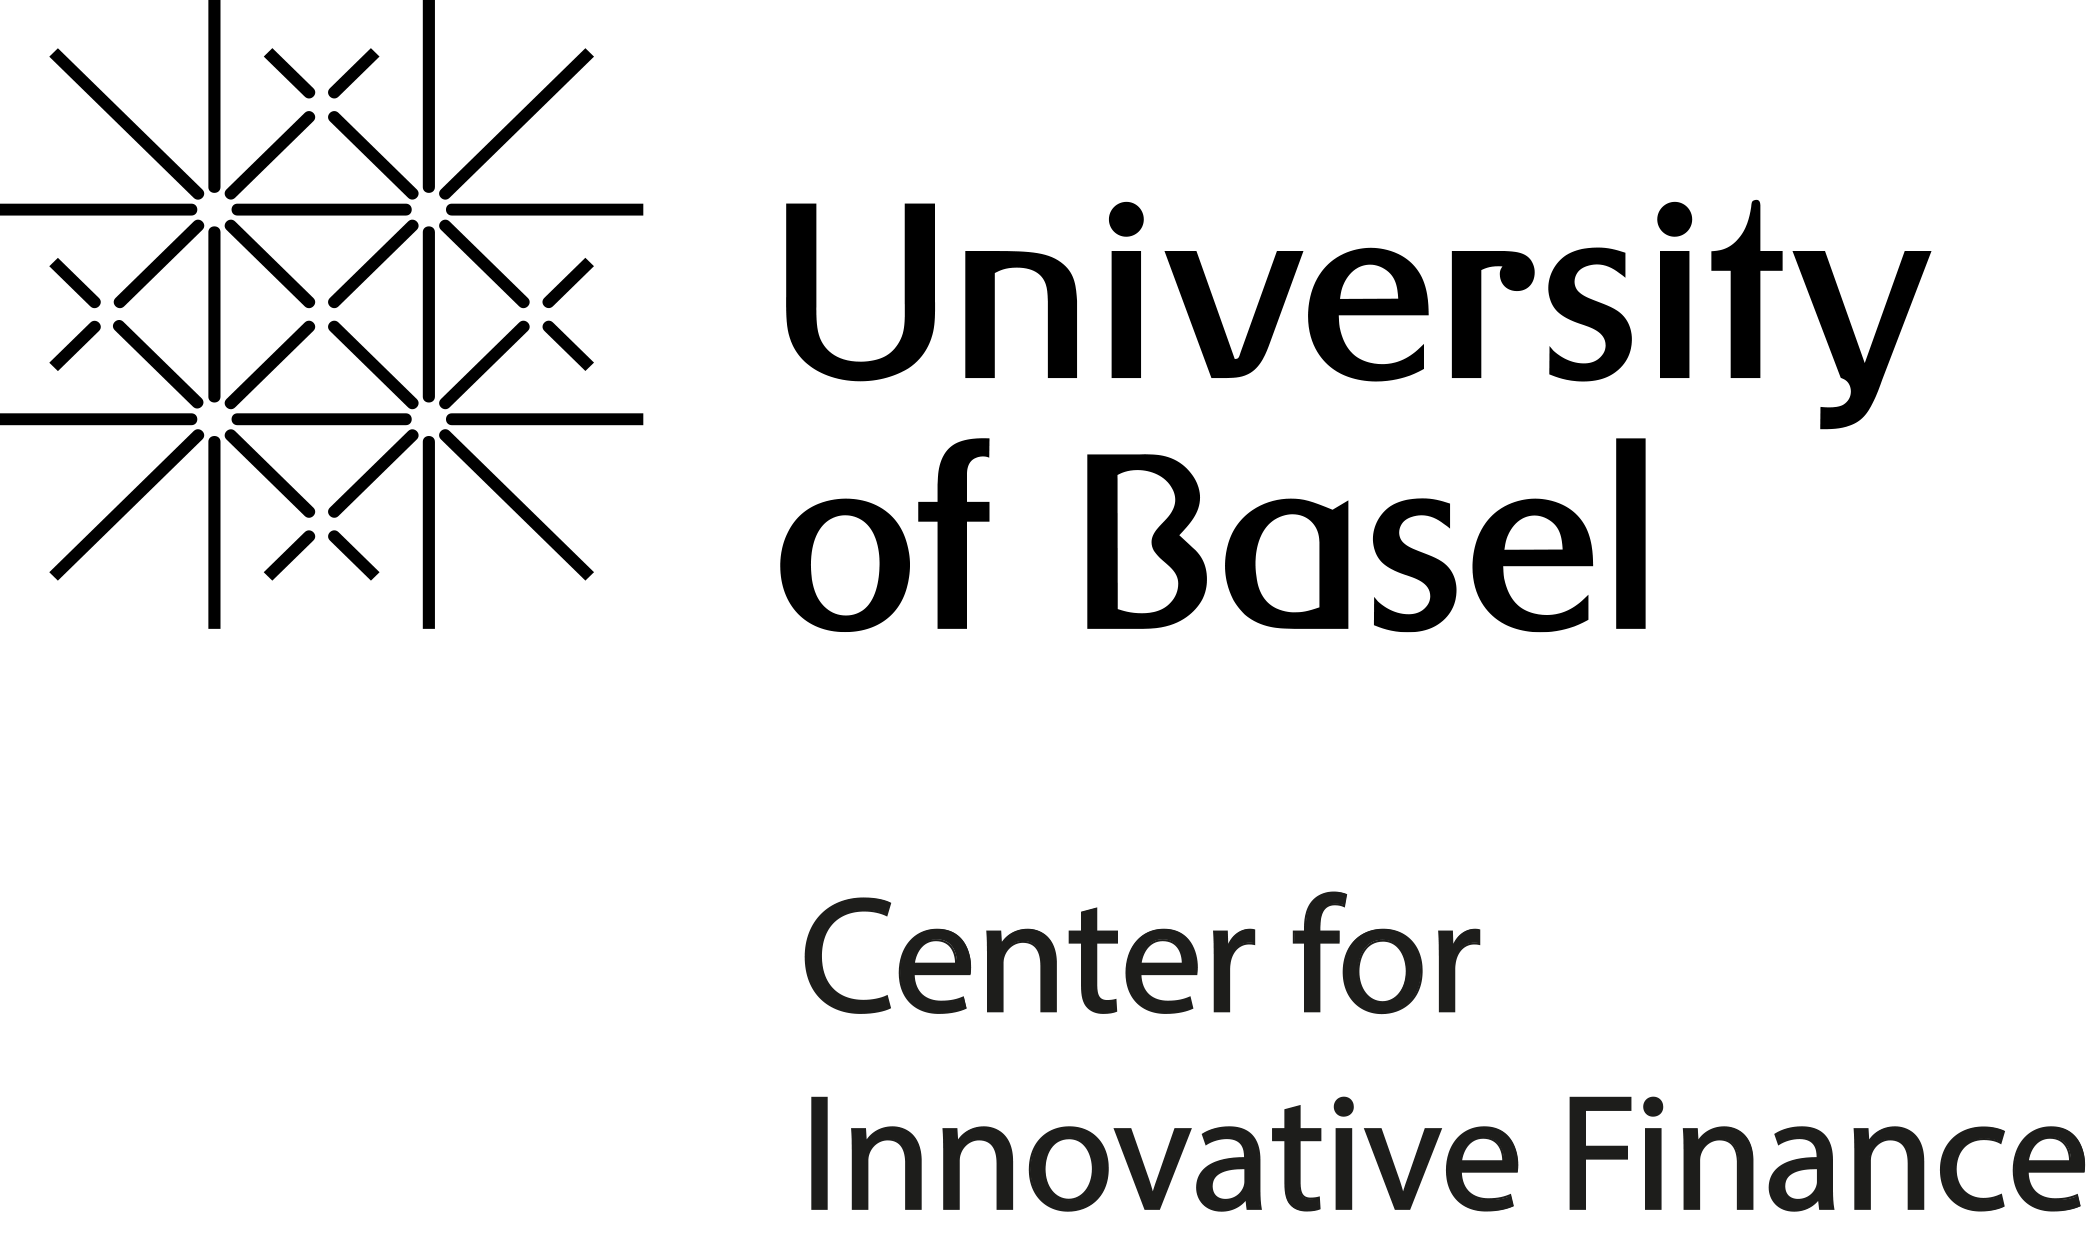
\includegraphics[width=2.5cm]{../config/logo_cif}
  
\includegraphics[width=1.9cm]{../config/seal_wwz}
  \\ \vspace{2em}
  \usebeamerfont{title}\textbf{\inserttitle}\par
  \usebeamerfont{title}\usebeamercolor[fg]{title}\insertsubtitle\par  \vspace{1.5em}
  \small\usebeamerfont{author}\insertauthor\par
  \usebeamerfont{author}\insertinstitute\par \vspace{2em}
  \usebeamercolor[fg]{titlegraphic}\inserttitlegraphic
    \tiny \noindent \texttt{Release Ver.: \gitRelease}\\ 
    \texttt{Version Hash: \gitSHA}\\
    \texttt{Version Date: \gitDate}\\ \vspace{1em}
  \link \href{https://github.com/cifunibas/Bitcoin-Blockchain-Cryptoassets/blob/main/slides/intro.pdf}
  {Get most recent version}\\
  \link \href{https://github.com/cifunibas/Bitcoin-Blockchain-Cryptoassets/blob/main/slides/intro.pdf}
  {Watch video lecture}\\ \vspace{1em}
  License: \texttt{Creative Commons Attribution-NonCommercial-ShareAlike 4.0 International}\\\vspace{2em}
  
\includegraphics[width = 1.2cm]{../config/license}
}

% tikzlibraries
\usetikzlibrary{decorations.pathreplacing}
\usetikzlibrary{decorations.markings}
\usetikzlibrary{positioning}

%caption font
\captionsetup{font=footnotesize}


%%%%%%%%%%%%%%%%%%%%%%%%%%%%%%%%%%%%%%%%%%%%%%
%%%%%%%%%%%%%%%%%%%%%%%%%%%%%%%%%%%%%%%%%%%%%%
\begin{document}

\thispagestyle{empty}
\begin{frame}[noframenumbering]
	\titlepage
\end{frame}

%%%
\begin{frame}{Diffie-Hellman-Merkle Key Exchange}
	\begin{itemize}
		\item<1-> Whitfield Diffie, Martin Hellman and Ralph Merkle find a solution for the \textit{key distribution} problem (1976)
		\item<2-> They still use symmetric encryption. However, the key can be generated securely on a potentially compromised channel. 
		\vspace{0.5cm}
		\item<3-> Alice and Bob define ex-ante
		\begin{itemize}
			\item<4-> One-way function: $Y^x\ (mod\ P)$
			\item<5-> Parameters: $Y = 7$ and $P = 11$
		\end{itemize}
	\end{itemize}
\end{frame}
%%%

%%%
\begin{frame}{Diffie-Hellman-Merkle Key Exchange}
	\begin{table}
		\centering
		\resizebox{10.5cm}{!}{
			\begin{tabular}{c c c c}
				\hline
				&Alice&&Bob\\
				\hline
				&&&\\
				Step 1 & chooses $A = 3$ && chooses $B = 6$\\
				&&&\\
				Step 2 & $\alpha = Y^A\ (mod\ P)$ && $\beta = Y^B\ (mod\ P)$ \\					& $\alpha = 7^3\ (mod\ 11) = 2$ &&$\beta = 7^6\ (mod\ 11) = 4$ \\
				&&&\\
				Step 3 & Alice sends her result $\alpha = 2$ to Bob && Bob sends his result $\beta = 4$ to Alice \\
				&&&\\
				\textit{Exchange} & \multicolumn{3}{c}{\textit{The only exchange of information (not key!)}}\\
				&&&\\
				Step 4 & Alice computes $k = \beta^A\ (mod\ P)$ && Bob computes $k = \alpha^B\ (mod\ P)$ \\
				&$k = 4^3\ (mod\ 11) = 64\ (mod\ 11) = 9$ && $k = 2^6\ (mod\ 11) = 64\ (mod\ 11) = 9$ \\
				&&&\\
				\textit{Key} & \multicolumn{3}{c}{\textit{Alice and Bob have agreed on key $k = 9$, because:}}\\
				& \multicolumn{3}{c}{$\alpha^{B}\ (mod\ P) = Y^{AB}\ (mod\ P) = Y^{BA}\ (mod\ P) = \beta^{A}\ (mod\ P)$}\\
				&&&\\
				\hline
			\end{tabular}
			}
		\caption{Diffie-Hellman-Merkle-Key-Exchange. Based on \cite{singh1999}}
	\end{table}
\end{frame}
%%%

%%%
\begin{frame}{Issues}
	\vspace{-0.3cm}
	\begin{figure}
		\centering
		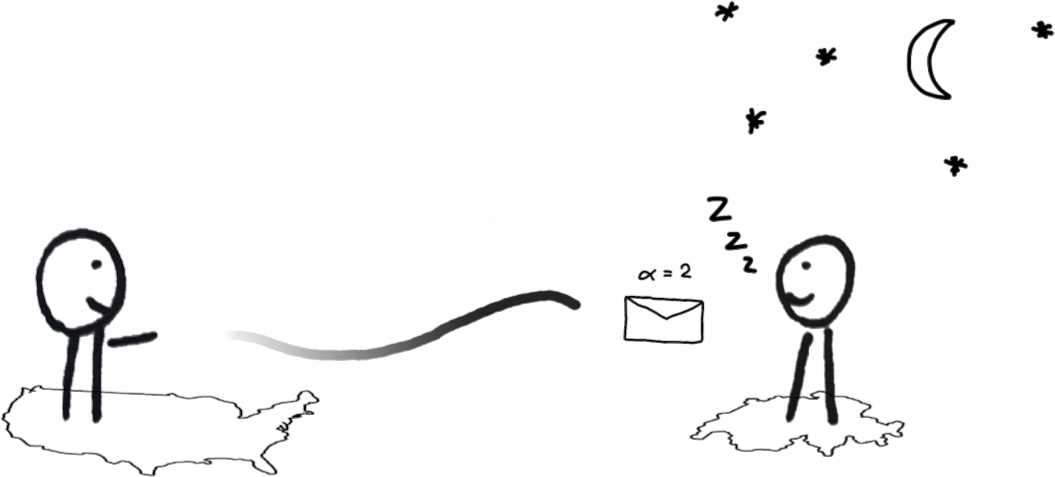
\includegraphics[width = 9cm]{../assets/images/drawing_DHM_exchange.png}
	\end{figure}
	\vspace{0.5cm}
	\begin{itemize}
		\item<1-> Undermines spontaneity of online communication
	\end{itemize}
\end{frame}
%%%

%%%
\begin{frame}{Asymmetric Cryptography}
	\begin{itemize}
		\item<1-> So far: Symmetric cryptography
		\begin{itemize}
			\item<1->Decryption is inverse algorithm of encryption
		\end{itemize}
		\item<2-> Diffie's Idea (1975): Asymmetric encryption
		\begin{itemize}
			\item<2->Key to encrypt and key to decrypt a message are not identical
		\end{itemize}
		\item<3->...but how?
	\end{itemize}
\end{frame}
%%%

%%%
\begin{frame}{Asymmetric Cryptography}
	\begin{itemize}
		\item<1-> Ronald Rivest, Adi Shamir and Leonard Adleman
		\item<2-> Inspired by Diffie's idea of asymmetric cryptography
		\item<3-> Develop first asymmetric encryption algorithm (\textit{RSA}) \cite{rivest1978}
	\end{itemize}
	\uncover<3->{
		\begin{figure}
			\centering
			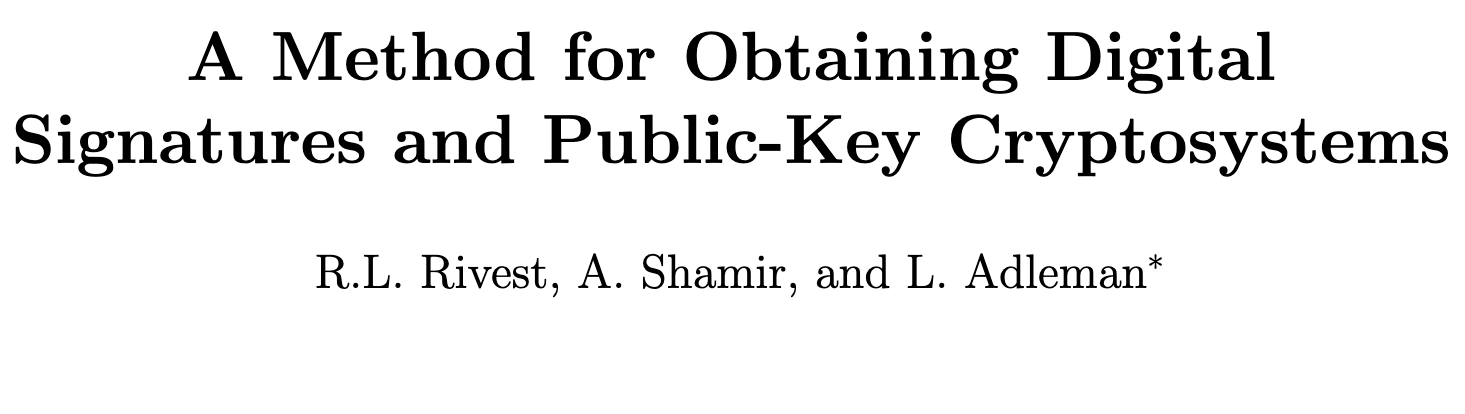
\includegraphics[width = 8cm]{../assets/images/cover_RSA}
		\end{figure}
	}
\end{frame}
%%%

%%%
\begin{frame}{RSA}
	Properties of asymmetric cryptography:
	\vspace{0.4cm}
	\begin{figure}
		\centering
		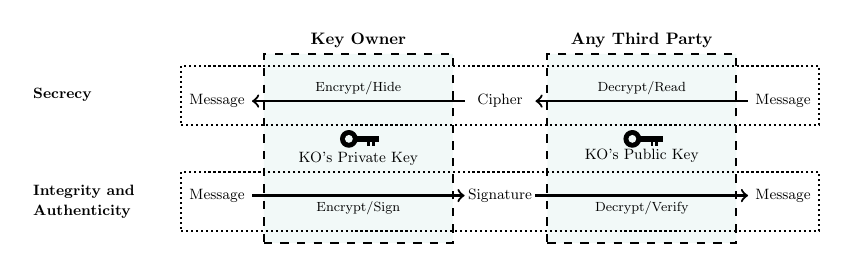
\begin{tikzpicture}[domain=-6:12,scale=0.6, every node/.style={scale=0.6}]
	
	\draw[fill= highlight!15, draw=black, thick, dashed] (0,0) -- (4,0) -- (4,4) -- (0,4) -- (0,0);
	\draw[fill= highlight!15, draw=black, thick, dashed] (6,0) -- (10,0) -- (10,4) -- (6,4) -- (6,0);
	
	\draw[draw=black, thick, densely dotted] (-1.75,2.5) -- (11.75,2.5) -- (11.75,3.75) -- (-1.75,3.75) -- (-1.75,2.5) node[left,midway,text width=3cm]{\small{\textbf{Secrecy}}};
	\draw[draw=black, thick, densely dotted] (-1.75,0.25) -- (11.75,0.25) -- (11.75,1.5) -- (-1.75,1.5) -- (-1.75,0.25)node[left,midway,text width=3cm]{\small{\textbf{Integrity and\\ Authenticity}}};
	
	
	
	\draw[<-,thick] (-0.25,3) -- (4.25,3) node[above, midway] {\footnotesize{Encrypt/Hide}};
	\draw[<-,thick] (5.75,3) -- (10.25,3) node[above, midway] {\footnotesize{Decrypt/Read}};
	
	\draw[->,thick] (-0.25,1) -- (4.25,1) node[below, midway] {\footnotesize{Encrypt/Sign}} ;
	\draw[->,thick] (5.75,1) -- (10.25,1) node[below, midway] {\footnotesize{Decrypt/Verify}} ;
	
	
	%\draw[<-,thick] (-0.3,3) -- node[above] {\footnotesize{Entschlüsselung}} ++(4.6,0);
	%\draw[<-,thick] (5.7,3) -- node[above] {\footnotesize{Verschlüsselung}} ++(4.6,0);
	
	%\draw[->,thick] (-0.3,1) -- node[below] {\footnotesize{Verschlüsseln/Signatur}} ++(4.6,0);
	%\draw[->,thick] (5.7,1) -- node[below] {\footnotesize{Entschlüsseln/Kontrolle}} ++(4.6,0);
	
	\draw  plot (5,3) node[]{\small{Cipher}};
	\draw  plot (5,1) node[]{\small{Signature}};
	
	\draw  plot (-0.99,3) node[]{\small{Message}};
	\draw  plot (-0.99,1) node[]{\small{Message}};
	
	\draw  plot (10.99,3) node[]{\small{Message}};
	\draw  plot (10.99,1) node[]{\small{Message}};
	
	%private key
	\filldraw[color=black] (1.8,2.2) circle (5pt) ;
	\filldraw[color=highlight!15] (1.8,2.2) circle (2pt);
	\filldraw[yshift=-0.05cm, xshift=0.1cm,color = black] (1.8,2.2) rectangle ++(15pt,3pt) ;
	\filldraw[yshift=-0.13cm, xshift=0.4cm,color = black] (1.8,2.2) rectangle ++(1pt,4pt) ;
	\filldraw[yshift=-0.13cm, xshift=0.5cm,color = black] (1.8,2.2) rectangle ++(1pt,4pt) ;
	\draw[color=black] plot (2,2.05) node[below] {\small{KO's Private Key}};
	\draw[color=black] plot (2,4) node[above] {\textbf{Key Owner}};
	
	%public key
	\filldraw[color=black] (7.8,2.2) circle (5pt);
	\filldraw[color=highlight!15] (7.8,2.2) circle (2pt);
	\filldraw[yshift=-0.05cm, xshift=0.1cm,color = black] (7.8,2.2) rectangle ++(15pt,3pt) ;
	\filldraw[yshift=-0.13cm, xshift=0.4cm,color = black] (7.8,2.2) rectangle ++(1pt,4pt) ;
	\filldraw[yshift=-0.13cm, xshift=0.5cm,color = black] (7.8,2.2) rectangle ++(1pt,4pt) ;
	\draw[color=black] plot (8,2.1) node[below] {\small{KO's Public Key}};
	\draw[color=black] plot (8,4) node[above] {\textbf{Any Third Party}};
	
\end{tikzpicture}
	\end{figure}
\end{frame}
%%%

%%%
\begin{frame}{RSA 1/4: Find Public Key}
	Alice chooses two primes $p$ and $q$ (e.g. $p = 17$ and $q = 11$) and computes
	\begin{align*}
		N &= p \cdot q \\
		\intertext{In our example:}
		\begin{split}
			N &= 17 \cdot 11 = 187 
		\end{split}
	\end{align*} 
	and choose an additional integer $e$ (e.g. $e = 7$).\footnote{\tiny $e$ and $(p-1)\cdot(q-1)$ have to be relative primes} \\
	\vspace{0.5cm}
	$\Rightarrow$ $N$ and $e$ together make up the public key which Alice can make publicly available.
\end{frame}
%%%

%%%
\begin{frame}{RSA 2/4: Encrypt Message}
	Bob encodes message $M$ as an integer (e.g. If $M =$ letter $X$ in ASCII $= 88$) and computes the encrypted message $C$ using Alice's public key and:  
	\begin{align*}
		C &= M^e\ (mod\ N) \\
		\intertext{In our example:}
		C &= 88^7\ (mod\ 187) \\
		C &= 11
	\end{align*}
\end{frame}
%%%

%%%
\begin{frame}{RSA 3/4: Derive Private Key}
	Alice computes private key $k_{p}$ using:
	\begin{align*}
		e \cdot k_{p} &= 1\ (mod\ \phi(N))\;\text{, where $\phi(N) = (p-1)(q-1)$}
		\intertext{In our example:}
		7 \cdot k_{p} &= 1\ (mod\ 16 \cdot 10) = 1\ (mod\ 160) \\
		k_{p} &= 23
	\end{align*}
	\uncover<2->{Note: Extended Euclidean algorithm is needed for this step}
\end{frame}
%%%

%%%
\begin{frame}{RSA 4/4: Decrypt Message}
	\begin{align*}
		\intertext{Alice decrypts Bob's message with:}
		M &= C^{k_{p}}\ (mod\ N)
		\intertext{and computes}
		M &= 11^{23}\ (mod\ 187) \\
		M &= 88 = X
		\text{\ in ASCII}
	\end{align*}
\end{frame}
%%%

%%%
\begin{frame}{RSA: Requirements}
	Crucial: 
	\begin{itemize}
		\item<1-> $N$ has to be sufficiently large
		\item<2-> It has to be impossible to find $p$ and $q$ by using prime factorization of $N$.
	\end{itemize}
\end{frame}
%%%

%%%
\begin{frame}{Pretty Good Privacy}
		\begin{itemize}
			\item<1->RSA is computationally costly
			\item<2->General public did not benefit 
			\item<3->Phil Zimmermann wanted to protect privacy of the average citizen on the internet as well
			\item<4->His solution: Pretty Good Privacy (PGP)
		\end{itemize}
\end{frame}
%%%

%%%
\begin{frame}{PGP: Workings}
	\begin{minipage}[T][5cm][t]{0.45\textwidth}
		Encryption:
		\begin{itemize}
			\item<1->Encryption of message is done symmetrically
			\item<2->Encryption of symmetric key using RSA-public-key of recipient
			\item<3->Sending encrypted message and symmetric key to recipient
		\end{itemize}
	\end{minipage}
	\hfill
	\begin{minipage}[T][5cm][t]{0.45\textwidth}
		\uncover<4->{Decryption:}
		\begin{itemize}
			\item<4->Decryption of symmetric key with RSA-private-key of recipient.
			\item<5->Decryption of message with decrypted symmetric key
		\end{itemize}
	\end{minipage}
\end{frame}
%%%

%%%
\begin{frame}%[allowframebreaks]
	\frametitle{References}
	\bibliographystyle{amsplain}
	\bibliography{../assets/bib/refs}
\end{frame}
%%%
\end{document}